\textbf{Partie A :}

\medskip

Soit $h$ la fonction définie sur $\R$ par $h(x) = \e^x-x$.

\begin{enumerate}
	\item Déterminer les limites de $h$ en $-\infty$ et $+\infty$.
	\item Étudier les variations de $h$ et dresser son tableau de variation.
	\item En déduire que :
	
	si $a$ et $b$ sont deux réels tels que $0 < a < b$ alors $h(a)-h(b) < 0$.
\end{enumerate}

\textbf{Partie B :}

\medskip

Soit $f$ la fonction définie sur $\R$ par $f(x) = \e^x$.

On note $\mathcal{C}_f$ sa courbe représentative dans un repère $\Rij$.

\begin{enumerate}
	\item Déterminer une équation de la tangente $\mathcal{T}$ à $\mathcal{C}_f$ au point d’abscisse 0.
\end{enumerate}

Dans la suite de l’exercice on s’intéresse à l’écart entre $\mathcal{T}$ et $\mathcal{C}_f$ au voisinage de 0. Cet écart est défini comme la différence des ordonnées des points de $\mathcal{T}$ et $\mathcal{C}_f$ de même abscisse.

\smallskip

On s’intéresse aux points d’abscisse $\frac{1}{n}$, avec $n$ entier naturel non nul.

On considère alors la suite $\suiten$ définie pour tout entier naturel non nul $n$ par : \[ u_n  = \exp\left(\dfrac{1}{n}\right)-\dfrac{1}{n}-1.\]
%
\begin{enumerate}[resume]
	\item Déterminer la limite de la suite $\suiten$.
	\item 
	\begin{enumerate}
		\item Démontrer que, pour tout entier naturel non nul $n$, \[ u_{n+1}-u_n = h \left( \dfrac{1}{n+1}\right) - h\left( \dfrac{1}{n}\right) \]%
		où $h$ est la fonction définie à la partie \textbf{A}.
		\item En déduire le sens de variation de la suite $\suiten$.
	\end{enumerate}
	\item Le tableau ci-dessous donne des valeurs approchées à $10^{-9}$ des premiers termes de la suite $\suiten$.
	
	\begin{center}
		\begin{tikzpicture}
			%\tabcolwidth{3cm}
			\tableur[11]{A-B}
			%colonneA
			\celtxt*[c]{A}{1}{$n$}
			\celtxt*[c]{A}{2}{1}
			\celtxt*[c]{A}{3}{2}
			\celtxt*[c]{A}{4}{3}
			\celtxt*[c]{A}{5}{4}
			\celtxt*[c]{A}{6}{5}
			\celtxt*[c]{A}{7}{6}
			\celtxt*[c]{A}{8}{7}
			\celtxt*[c]{A}{9}{8}
			\celtxt*[c]{A}{10}{9}
			\celtxt*[c]{A}{11}{10}
			%colonneB
			\celtxt*[c]{B}{1}{$v_n$}
			\celtxt*[c]{B}{2}{0,718281828}
			\celtxt*[c]{B}{3}{0,148721271}
			\celtxt*[c]{B}{4}{0,062279092}
			\celtxt*[c]{B}{5}{0,034025417}
			\celtxt*[c]{B}{6}{0,021402758}
			\celtxt*[c]{B}{7}{0,014693746}
			\celtxt*[c]{B}{8}{0,010707852}
			\celtxt*[c]{B}{9}{0,008148453}
			\celtxt*[c]{B}{10}{0,006407958}
			\celtxt*[c]{B}{11}{0,005170918}
		\end{tikzpicture}
	\end{center}
	%
	Donner la plus petite valeur de l’entier naturel $n$ pour laquelle l’écart entre $\mathcal{T}$ et $\mathcal{C}_f$ semble être inférieur à $10^{-2}$.
\end{enumerate}

